% ============================================================
%  BAB 3 — OBJEK DAN METODOLOGI PENELITIAN (REVISI LENGKAP)
%  NusaNara: Sistem Bimbingan Karier Berbasis RAG dan LLM
%  SEMUA GAMBAR: ekstrak dari PDF asli skripsi
% ============================================================
\chapter{OBJEK DAN METODOLOGI PENELITIAN}

Bab ini menguraikan secara rinci mengenai objek penelitian serta pendekatan dan prosedur
metodologis yang digunakan. Setiap tahapan, mulai dari rancangan sistem hingga teknik
analisis data, dijelaskan secara sistematis untuk memastikan penelitian ini dilaksanakan
dengan \textit{rigor} dan validitas yang tinggi.

% -------------------------------------------------------
\section{Objek Penelitian}
% -------------------------------------------------------
Objek penelitian ini adalah sebuah artefak komputasi berupa prototipe aplikasi web
fungsional yang diberi nama \textbf{``NusaNara''}. Artefak ini mencakup kode program,
keseluruhan arsitektur \textit{full-stack} yang dirancang, basis pengetahuan yang dikurasi,
serta alur interaksi pengguna yang diimplementasikan. Artefak inilah yang akan dievaluasi
untuk menjawab rumusan masalah penelitian.

% -------------------------------------------------------
\section{Metodologi Penelitian}
% -------------------------------------------------------
Penelitian ini mengadopsi pendekatan \textit{Design Science Research} (DSR) yang dimulai
dari \textit{entry point} yang berpusat pada masalah (\textit{problem-centered initiation}),
di mana identifikasi masalah nyata di lapangan menjadi pemicu utama. Pemilihan DSR
didasarkan pada argumen bahwa fokus penelitian ini adalah pada penciptaan solusi (sebuah
sistem baru), bukan pada deskripsi atau eksplanasi fenomena yang sudah ada \cite{Peffers2007}.

Alur penelitian mengikuti enam fase utama DSR, sebagaimana diilustrasikan pada Gambar \ref{fig:dsr_tahapan}:

\begin{figure}[H]
  \centering
  
\includegraphics[width=0.95\textwidth]{gambar_3_1_dsr_tahapan}
  \caption{Tahapan \textit{Design Science Research} (DSR) (Sumber: Peffers et al., 2007)}
  \label{fig:dsr_tahapan}
\end{figure}

\begin{enumerate}
  \item \textbf{Identifikasi Masalah:} Melakukan studi literatur untuk memvalidasi urgensi
    masalah dan merumuskan pertanyaan penelitian. Didukung oleh data BPS \cite{BPS2025} yang
    menunjukkan TPT lulusan SMK tertinggi sebesar 8,10\%, serta survei kebutuhan terhadap
    115 responden aktif.

  \item \textbf{Perumusan Tujuan:} Menentukan kebutuhan fungsional solusi: sistem yang
    mampu memproses narasi karier pengguna secara alami, meretrieve konteks faktual dari
    720 lowongan pekerjaan, dan menghasilkan rekomendasi yang terstruktur dan dapat
    ditelusuri (\textit{traceable}).

  \item \textbf{Perancangan \& Pengembangan Artefak:} Membangun prototipe fungsional
    ``NusaNara'' secara iteratif menggunakan metode \textit{prototype}, berdasarkan
    arsitektur \textit{full-stack} yang dirancang spesifik untuk mengimplementasikan alur
    RAG dengan \textit{Hybrid Search} secara efisien (lihat Gambar \ref{fig:arsitektur_sistem}).

  \item \textbf{Demonstrasi:} Uji teknis melalui \textit{black-box testing} untuk
    memvalidasi alur fungsi utama, memastikan stabilitas, dan memperbaiki \textit{bug}
    kritikal sebelum evaluasi formal.

  \item \textbf{Evaluasi:} Evaluasi artefak menggunakan pendekatan empat lapis:
    (a) evaluasi teknis retrieval (P@k, MRR), (b) pengujian fungsional \textit{black-box},
    (c) evaluasi kinerja sistem (latensi), dan (d) evaluasi penerimaan pengguna (UAT Likert).

  \item \textbf{Komunikasi:} Menganalisis dan mendokumentasikan seluruh temuan penelitian
    dalam laporan skripsi.
\end{enumerate}

% -------------------------------------------------------
\section{Jenis Artefak Penelitian}
% -------------------------------------------------------
Sesuai taksonomi artefak DSR \cite{Peffers2007}, penelitian ini menghasilkan tiga jenis artefak:

\begin{enumerate}
  \item \textbf{Model (Arsitektur Konseptual):} Cetak biru arsitektur \textit{full-stack}
    yang merinci orkestrasi antara empat lapisan utama:
    \begin{itemize}[noitemsep]
      \item \textit{Frontend}: Next.js 14 (TypeScript) dengan \texttt{@microsoft/fetch-event-source} dan Clerk Auth
      \item \textit{Backend}: FastAPI + Uvicorn (ASGI), pipeline RAG lengkap, Clerk JWT validator
      \item \textit{Database}: PostgreSQL 16 + pgvector (VECTOR(768)) + tsvector FTS
      \item \textit{Local AI}: Ollama (Llama 3.1 8B (4-bit Quantized) sebagai generator \& extractor agent;
        nomic-embed-text-v2-moe sebagai model embedding 768 dimensi)
    \end{itemize}

  \item \textbf{Instantiation (Implementasi Fisik):} Prototipe fungsional aplikasi web
    ``NusaNara'' yang berjalan di produksi (VPS Ubuntu + Vercel), sebagai bukti nyata
    bahwa arsitektur yang diusulkan dapat diimplementasikan secara teknis.

  \item \textbf{Method (Alur Kerja Terstruktur):} Metodologi evaluasi empat lapis yang
    menggabungkan evaluasi teknis RAG (P@k, MRR), pengujian fungsional \textit{black-box},
    evaluasi latensi sistem, dan UAT dengan instrumen Likert.
\end{enumerate}

% -------------------------------------------------------
\section{Rancangan Penelitian}
% -------------------------------------------------------
\subsection{Subjek dan Lokasi Penelitian}
Populasi target adalah mahasiswa aktif dan siswa tingkat akhir (SMA/SMK) di Indonesia
yang berada dalam fase eksplorasi dan pengambilan keputusan karier. Sampel terdiri dari
dua kelompok:

\begin{enumerate}
  \item \textbf{Pengguna Akhir:} 10--15 mahasiswa aktif dipilih menggunakan teknik
    \textit{purposive sampling} berdasarkan kriteria: sedang dalam fase eksplorasi karier
    aktif (minimal semester 5 atau sedang mencari pekerjaan pertama). Teknik ini dipilih
    karena tujuan evaluasi adalah memvalidasi kegunaan artefak pada konteks yang dituju,
    bukan generalisasi statistik ke populasi \cite{Peffers2007}.

  \item \textbf{Pengumpulan Data Kebutuhan Awal:} 115 responden (mahasiswa dan siswa)
    telah dilibatkan dalam survei kuantitatif awal untuk memvalidasi masalah dan
    memprioritaskan fitur sistem.
\end{enumerate}

Seluruh proses pengumpulan data dilaksanakan secara daring (\textit{remote}), memanfaatkan
Google Form sebagai instrumen, sehingga memungkinkan jangkauan partisipan yang lebih luas.

\subsection{Teknik Pengumpulan Data}
Pengumpulan data dilaksanakan melalui tiga alur utama:

\paragraph{Alur 1: Survei Kebutuhan Awal (115 Responden)}
Tahap ini bertujuan memvalidasi masalah dan memprioritaskan kebutuhan sistem secara
kuantitatif. Instrumen berupa kuesioner daring terstruktur mencakup:
\begin{itemize}[noitemsep]
  \item Validasi masalah: Skala Likert untuk mengukur tingkat kesulitan dalam pengambilan
    keputusan karier dan kecemasan fenomena ``salah jurusan''.
  \item Prioritas kebutuhan: responden memberi peringkat (\textit{rank-order}) fitur
    potensial (rekomendasi naratif, kemampuan adaptif, data lokal).
\end{itemize}
Data survei ini telah berhasil dikumpulkan dengan total \textbf{115 responden}.

\paragraph{Alur 2: Pengumpulan Data Konten untuk Knowledge Base}
Alur ini difokuskan pada pengumpulan data lowongan pekerjaan sebagai basis pengetahuan RAG.
Pada tahap awal, tiga platform karier dievaluasi: Jobstreet, LinkedIn, dan Glints.
Evaluasi menemukan:

\begin{itemize}[noitemsep]
  \item \textbf{Jobstreet:} menerapkan proteksi \textit{bot-detection} berbasis Cloudflare
    yang memblokir permintaan otomatis secara konsisten.
  \item \textbf{LinkedIn:} tidak menampilkan informasi gaji secara publik -- atribut yang
    relevan untuk analisis pasar kerja kontekstual.
  \item \textbf{Glints:} aksesibel secara teknis dan menyediakan atribut data yang lengkap.
\end{itemize}

Berdasarkan evaluasi ini, \textbf{Glints dipilih sebagai satu-satunya sumber data}.
Scraping dilakukan menggunakan Selenium WebDriver dengan konfigurasi \textit{selenium-stealth},
diperlukan karena Glints merupakan \textit{Single Page Application} (SPA) berbasis React
yang mengandalkan JavaScript untuk merender konten.

Hasil akhir: \textbf{720 lowongan pekerjaan} berhasil dikumpulkan pada periode akhir \textbf{April 2026} (tepatnya 30 April 2026), terdistribusi ke dalam \textbf{8 klaster karier},
masing-masing klaster berisi tepat \textbf{90 lowongan}. Distribusi seimbang ini merupakan
persyaratan metodologis utama untuk memastikan validitas evaluasi RAG yang adil lintas
seluruh domain karier.

\begin{table}[H]
\centering
\caption{Distribusi \textit{Knowledge Base} Berdasarkan 8 Klaster Karier}
\label{tab:klaster}
\begin{tabular}{clc}
\toprule
\textbf{No} & \textbf{Klaster Karier} & \textbf{Jumlah Lowongan} \\
\midrule
1 & Teknologi \& Perangkat Lunak & 90 \\
2 & Analisis Data & 90 \\
3 & Desain \& Kreatif & 90 \\
4 & Pemasaran Digital & 90 \\
5 & Bisnis \& Administrasi & 90 \\
6 & Sales \& Customer Service & 90 \\
7 & Finance \& Accounting & 90 \\
8 & Education \& Training & 90 \\
\midrule
\multicolumn{2}{l}{\textbf{Total}} & \textbf{720} \\
\bottomrule
\end{tabular}
\end{table}

\paragraph{Alur 3: Pengumpulan Data Evaluasi (UAT)}
Setelah prototipe mencapai status stabil, data evaluasi penerimaan pengguna dikumpulkan
menggunakan kuesioner 7 pertanyaan Skala Likert (1--5) dari 10--15 responden (lihat
Sub-bab \ref{subsec:analisis_data}).

\subsection{Teknik Pengembangan Sistem}
Pengembangan sistem dilakukan secara iteratif menggunakan metode \textit{prototype}.

\begin{figure}[H]
  \centering
  
\includegraphics[width=0.80\textwidth]{gambar_3_3_prototype}
  \caption{Alur Metode \textit{Prototype} (Sumber: Kholis \& Zaky, 2025)}
  \label{fig:prototype_flow}
\end{figure}

Tahapan pengembangan:

\begin{enumerate}
  \item \textbf{Pengumpulan Kebutuhan:} Dua alur paralel -- (a) \textit{User-Centric}:
    analisis survei 115 responden; (b) \textit{Data-Centric}: scraping 720 lowongan dari Glints.

  \item \textbf{Perancangan Desain:} Kebutuhan diterjemahkan menjadi arsitektur \textit{full-stack}:
    Next.js 14 (frontend), FastAPI (backend), PostgreSQL 16 + pgvector (database),
    Ollama + Llama 3.1 (LLM), dan \textit{Adaptive Profile System} (personalisasi).

  \item \textbf{Perancangan Prototipe:} Implementasi komponen inti: FastAPI + RAG pipeline,
    PostgreSQL + pgvector, Ollama (Llama 3.1 + nomic-embed), Next.js 14, dan Clerk JWT.

  \item \textbf{Uji Coba \& Evaluasi Formatif:} \textit{Black-box testing} internal oleh
    peneliti untuk memverifikasi fungsionalitas dan memperbaiki \textit{bug} kritikal.
\end{enumerate}

\subsubsection{Kode Logika Web Scraping Glints}

Berikut adalah kode Python inti dari skrip scraping Glints yang digunakan untuk
mengumpulkan data 720 lowongan pekerjaan. Konfigurasi \textit{selenium-stealth}
diperlukan untuk mengelabui deteksi bot pada SPA berbasis React:

\begin{lstlisting}[language=Python, caption={Logika inti scraping Glints dengan Selenium Stealth}]
import time, json, csv
from selenium import webdriver
from selenium.webdriver.chrome.options import Options
from selenium.webdriver.common.by import By
from selenium_stealth import stealth

def create_stealth_driver():
    """Inisialisasi Chrome WebDriver dengan konfigurasi anti-deteksi."""
    options = Options()
    options.add_argument("--headless")
    options.add_argument("--no-sandbox")
    options.add_argument("--disable-dev-shm-usage")
    driver = webdriver.Chrome(options=options)
    # Konfigurasi stealth: sembunyikan tanda-tanda otomasi WebDriver
    stealth(driver,
        languages=["id-ID", "id"],
        vendor="Google Inc.",
        platform="Win32",
        webgl_vendor="Intel Inc.",
        fix_hairline=True,
    )
    return driver

def scrape_glints_cluster(cluster_name, search_query, target_count=90):
    """Scraping lowongan untuk satu klaster karier dari Glints."""
    driver = create_stealth_driver()
    jobs = []
    page = 1
    base_url = f"https://glints.com/id/opportunities/jobs/explore"

    while len(jobs) < target_count:
        url = f"{base_url}?keyword={search_query}&page={page}"
        driver.get(url)
        time.sleep(3)  # Tunggu SPA render (JavaScript)

        # Ambil kartu lowongan setelah JS render selesai
        job_cards = driver.find_elements(By.CSS_SELECTOR, "[data-cy='job-card']")
        if not job_cards:
            break  # Tidak ada lowongan tersisa

        for card in job_cards:
            try:
                job = {
                    'cluster':  cluster_name,
                    'title':    card.find_element(By.CSS_SELECTOR, "h2").text,
                    'company':  card.find_element(By.CSS_SELECTOR, "[data-cy='company-name']").text,
                    'location': card.find_element(By.CSS_SELECTOR, "[data-cy='job-location']").text,
                    'skills':   [s.text for s in card.find_elements(By.CSS_SELECTOR, "[data-cy='job-skill']")],
                    'salary':   card.find_element(By.CSS_SELECTOR, "[data-cy='salary-range']").text,
                }
                jobs.append(job)
            except Exception:
                continue  # Skip kartu yang tidak lengkap

        if len(jobs) >= target_count:
            break
        page += 1

    driver.quit()
    return jobs[:target_count]  # Pastikan tepat 90 per klaster

# Eksekusi untuk semua 8 klaster
CLUSTERS = {
    'Teknologi & Perangkat Lunak': 'software engineer',
    'Analisis Data':               'data analyst',
    'Desain & Kreatif':            'UI UX designer',
    'Pemasaran Digital':           'digital marketing',
    'Bisnis & Administrasi':       'business analyst',
    'Sales & Customer Service':    'sales customer service',
    'Finance & Accounting':        'finance accounting',
    'Education & Training':        'education trainer',
}

all_jobs = []
for cluster, query in CLUSTERS.items():
    print(f"Scraping: {cluster}...")
    cluster_jobs = scrape_glints_cluster(cluster, query, target_count=90)
    all_jobs.extend(cluster_jobs)
    print(f"  -> {len(cluster_jobs)} lowongan terkumpul")

print(f"Total: {len(all_jobs)} lowongan dari {len(CLUSTERS)} klaster")
# Output: Total: 720 lowongan dari 8 klaster
\end{lstlisting}

\subsubsection{Pipeline Pembersihan dan Embedding Data}

Setelah proses scraping menghasilkan 720 dokumen mentah, dua tahap pra-pemrosesan
dilakukan sebelum data siap digunakan oleh sistem RAG. Alur arsitektur pipeline pembersihan
dan *indexing* data dapat dilihat pada Gambar \ref{fig:pipeline_cleaning}.

\begin{figure}[H]
  \centering
  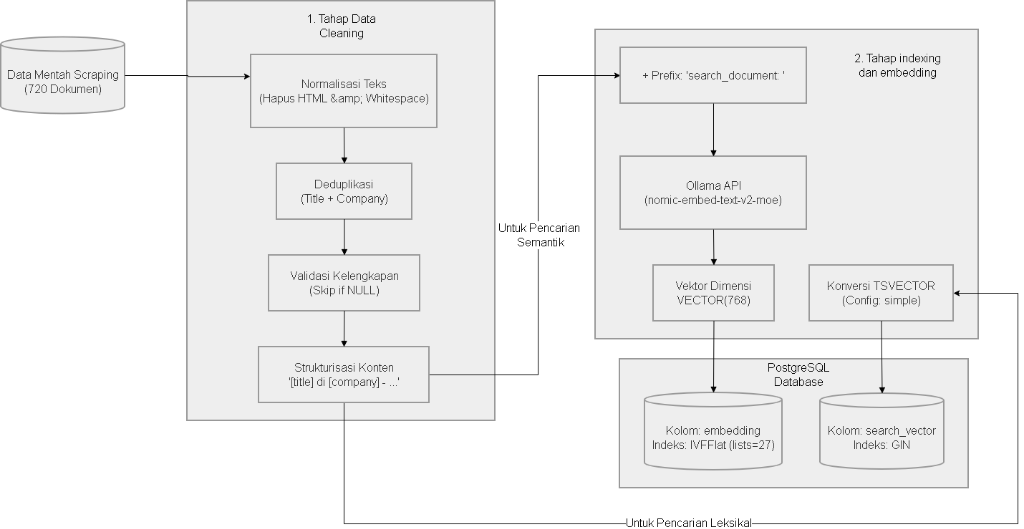
\includegraphics[width=\textwidth]{figures/gambar_3_6_pipeline.png}
  \caption{Arsitektur Pipeline Pembersihan Data dan Indexing Vektor (ETL)}
  \label{fig:pipeline_cleaning}
\end{figure}

\textbf{Tahap 1 --- Pembersihan Data (\textit{Data Cleaning}):}
Setiap dokumen mentah dibersihkan menggunakan pipeline otomatis:
\begin{itemize}[noitemsep]
  \item \textbf{Normalisasi teks:} Menghapus karakter HTML (\texttt{<br>}, \texttt{\&amp;}),
    whitespace berlebih, dan karakter non-printable.
  \item \textbf{Deduplikasi:} Mendeteksi dan menghapus lowongan duplikat berdasarkan
    kombinasi (title + company). Dari 720 hasil scraping, tidak ditemukan duplikat
    karena setiap klaster menggunakan keyword pencarian yang berbeda.
  \item \textbf{Validasi kelengkapan:} Memastikan setiap dokumen memiliki minimal
    field: title, company, dan skills. Dokumen dengan field kosong di-\textit{skip}.
  \item \textbf{Strukturisasi konten:} Setiap dokumen diformat menjadi teks gabungan
    yang mengombinasikan seluruh field: ``[title] di [company] - [location].
    Skills: [skills].'' Format ini memastikan informasi
    penting tertangkap dalam satu blok teks untuk proses embedding.
\end{itemize}

\textbf{Tahap 2 --- Generasi Embedding dan Indexing:}
Setiap dokumen yang telah dibersihkan dikonversi menjadi vektor 768 dimensi menggunakan
model \texttt{nomic-embed-text-v2-moe} via Ollama API:

\begin{equation}
  \mathbf{v}_d = f_{embed}(\texttt{``search\_document: ''} \| content_d) \in \mathbb{R}^{768}
  \label{eq:doc_embedding}
\end{equation}

\noindent Prefix \texttt{search\_document:} membedakan dokumen dari query (yang
menggunakan \texttt{search\_query:}), memungkinkan model menghasilkan representasi
yang dioptimalkan untuk masing-masing peran.

Vektor embedding disimpan ke kolom \texttt{knowledge\_base.embedding} bertipe
\texttt{VECTOR(768)}, dan diindeks menggunakan algoritma \textbf{IVFFlat}
dengan parameter \texttt{lists = 27} (jumlah cluster K-Means = $\sqrt{720} \approx 26.8$,
dibulatkan ke atas). Parameter ini mengikuti rekomendasi pgvector official documentation.

Secara paralel, kolom \texttt{search\_vector} bertipe \texttt{TSVECTOR} di-generate
dari teks konten menggunakan konfigurasi \texttt{simple} (tanpa stemming bahasa tertentu,
karena konten mengandung campuran bahasa Indonesia dan Inggris). Indeks GIN
dibuat pada kolom ini untuk pencarian leksikal cepat.

\subsection{Arsitektur Sistem}
\label{subsec:arsitektur}

Arsitektur sistem NusaNara mengadopsi pendekatan \textbf{Unified Database Architecture}
yang menempatkan PostgreSQL 16 sebagai satu-satunya sistem penyimpanan data.
Berbeda dengan pendekatan \textit{multi-database} yang lazim digunakan dalam sistem RAG
konvensional --- di mana penyimpanan vektor (misalnya ChromaDB, Pinecone, atau Weaviate)
dipisahkan dari penyimpanan relasional --- arsitektur ini memanfaatkan ekstensi
\textbf{pgvector} untuk mengintegrasikan kapabilitas penyimpanan dan pencarian vektor
secara \textit{native} di dalam PostgreSQL.

Keuntungan utama pendekatan \textit{Unified Database} ini adalah:
\begin{itemize}
  \item \textbf{Konsistensi transaksional (ACID):} Seluruh operasi --- menyimpan dokumen,
    vektor embedding, profil pengguna, dan riwayat rekomendasi --- dijamin konsisten
    dalam satu transaksi database. Tidak ada risiko \textit{data drift} antar sistem.
  \item \textbf{Eliminasi sinkronisasi:} Pendekatan multi-database memerlukan mekanisme
    sinkronisasi yang menambah kompleksitas operasional dan titik kegagalan.
  \item \textbf{Simplifikasi deployment:} Hanya satu proses database yang perlu
    di-\textit{manage}, di-\textit{backup}, dan di-\textit{monitor} di VPS.
  \item \textbf{Hybrid Search dalam satu query:} Pencarian semantik (pgvector) dan
    pencarian leksikal (tsvector) dapat digabungkan dalam satu \textit{query plan}
    PostgreSQL tanpa \textit{network hop} antar layanan.
\end{itemize}

\begin{figure}[H]
  \centering
  
\includegraphics[width=\textwidth]{arsitektur_sistem}
  \caption{Arsitektur Sistem NusaNara}
  \label{fig:arsitektur_sistem}
\end{figure}

Sebagaimana diilustrasikan pada Gambar \ref{fig:arsitektur_sistem}, sistem terdiri dari
empat lapisan yang terintegrasi:

\subsubsection{Lapisan 1: Antarmuka Pengguna (Next.js 14)}
Lapisan antarmuka dibangun menggunakan Next.js 14 dengan arsitektur \textit{Pages Router} dan JavaScript/JSX.
Komponen utama:
\begin{itemize}
  \item \textbf{fetch-event-source API:} Komponen React yang membuka koneksi SSE
    (\textit{Server-Sent Events}) ke endpoint \texttt{POST /api/recommend}.
    SSE dipilih (bukan WebSocket) karena alur komunikasi bersifat \textit{unidirectional} ---
    server mengirimkan token secara bertahap ke klien tanpa memerlukan respons balik
    selama proses streaming berlangsung. Protokol SSE juga lebih sederhana untuk
    di-\textit{proxy} melalui Nginx dibandingkan WebSocket yang memerlukan
    \textit{connection upgrade}.
  \item \textbf{Autentikasi Clerk v7 \& Token Caching:} Setiap halaman dilindungi menggunakan
    komponen proteksi standar dari Clerk. Token JWT disisipkan ke header
    \texttt{Authorization: Bearer <token>} pada setiap permintaan API ke backend.
    Untuk mengatasi isu pengambilan ulang (\textit{regenerate}) token yang berlebihan akibat siklus render React,
    sistem mengimplementasikan sebuah \textit{module-level token cache}. Cache ini menyimpan token 
    beserta waktu kedaluwarsanya di memori modul sehingga token yang sama (dengan konfigurasi \textit{lifetime} khusus)
    dapat terus digunakan pada setiap permintaan API baru selama masa berlakunya masih memenuhi ambang batas 5 menit.
    Backend memverifikasi token ini secara independen.
  \item \textbf{Halaman Riwayat:} Menampilkan seluruh sesi rekomendasi sebelumnya,
    memungkinkan pengguna melacak perkembangan eksplorasi karier dari waktu ke waktu.
\end{itemize}

\subsubsection{Lapisan 2: Logika Bisnis (FastAPI Backend)}
Seluruh pipeline RAG dieksekusi pada lapisan ini. FastAPI dipilih karena dukungan
\textit{native} terhadap \texttt{async/await} (ASGI via Uvicorn), yang krusial untuk:
(1) koneksi database asyncpg yang sepenuhnya asinkron memerlukan \textit{event loop}, dan
(2) streaming respons LLM via \texttt{StreamingResponse} memerlukan generator asinkron
(\texttt{async def generate()}) yang menghasilkan token satu per satu.
Pipeline terdiri dari 8 tahap yang dijelaskan pada Sub-bab \ref{subsec:pipeline_detail}.

\subsubsection{Lapisan 3: Penyimpanan Data (PostgreSQL 16 + pgvector)}
PostgreSQL 16 menyimpan seluruh data dalam tiga tabel utama:
\begin{itemize}
  \item \texttt{knowledge\_base}: 720 dokumen lowongan dengan kolom \texttt{embedding}
    bertipe \texttt{VECTOR(768)} yang diindeks menggunakan algoritma \textbf{IVFFlat}
    (\textit{Inverted File with Flat quantization}). IVFFlat membagi ruang vektor
    menjadi \textit{cluster} menggunakan K-Means, sehingga pencarian ANN
    (\textit{Approximate Nearest Neighbor}) hanya perlu memeriksa \textit{cluster}
    terdekat --- bukan seluruh 720 vektor. Kolom \texttt{search\_vector} bertipe
    \texttt{TSVECTOR} diindeks dengan GIN (\textit{Generalized Inverted Index})
    untuk pencarian leksikal cepat.
  \item \texttt{user\_profiles}: Profil adaptif yang diperbarui akumulatif oleh
    \textit{Extractor Agent}. Kolom \texttt{identified\_skills} dan
    \texttt{career\_interests} bertipe \texttt{TEXT[]} (array PostgreSQL).
  \item \texttt{recommendation\_history}: Log lengkap setiap sesi rekomendasi,
    mencakup narasi input, profil saat itu, dokumen yang di-retrieve, dan output LLM.
\end{itemize}

\subsubsection{Lapisan 4: Inferensi Lokal (Ollama)}
Ollama menjalankan dua model AI secara lokal di VPS:
\begin{itemize}
  \item \textbf{Llama 3.1 8B (4-bit Quantized):} Digunakan untuk dua peran ---
    (a) \textit{Main RAG Agent}: menghasilkan rekomendasi karier 5 seksi terstruktur
    berdasarkan konteks Top-3 dokumen; dan (b) \textit{Extractor Agent}: mengekstrak
    skill, minat, dan ringkasan dari narasi pengguna ke format JSON.
    Pemilihan model versi 8B dengan teknik kuantisasi 4-bit (Q4\_K\_M) merupakan keputusan
    teknis agar sesuai dengan keterbatasan memori VPS (16 GB RAM). Ollama secara efisien
    me-\textit{load} bobot model $\sim$5 GB satu kali ke dalam memori. Ketika dua agen
    berjalan bergantian, keduanya berbagi \textit{instance} model yang sama tanpa
    menggandakan konsumsi memori, menyisakan cukup memori untuk PostgreSQL
    ($\sim$2 GB \textit{shared buffers}) dan proses sistem operasi.
  \item \textbf{nomic-embed-text-v2-moe (768 dimensi):} Model embedding berbasis
    \textit{Mixture of Experts} (MoE) yang mengaktifkan subset dari parameter untuk
    setiap input, menghasilkan representasi vektor yang lebih efisien. Penggunaan
    prefix \texttt{search\_query:} dan \texttt{search\_document:} telah dijelaskan
    pada tahap \textit{embedding} pipeline ETL (Sub-bab sebelumnya).
\end{itemize}

% -------------------------------------------------------
\subsection{Analisis Kompleksitas Komputasional Pipeline RAG}
\label{subsec:kompleksitas}
% -------------------------------------------------------

Analisis kompleksitas waktu ($O$-notation) penting untuk memahami skala performa
sistem saat jumlah dokumen atau pengguna meningkat.

\begin{table}[H]
\centering
\caption{Analisis Kompleksitas Komputasional Per Tahap Pipeline RAG}
\label{tab:kompleksitas}
\begin{tabularx}{\textwidth}{clXl}
\toprule
\textbf{Tahap} & \textbf{Operasi} & \textbf{Keterangan} & \textbf{Big-O} \\
\midrule
1 & Query Expansion & Pencarian dalam dict statis 8 klaster & $O(1)$ \\
2 & Embedding & Inferensi model nomic-embed (konstan) & $O(L)$ \\
3 & Semantic Search & IVFFlat ANN (bukan brute-force) & $O(\sqrt{n})$ \\
4 & Lexical Search & Indeks GIN inverted & $O(\log n + m)$ \\
5 & RRF Fusion & Merge dua list 20 item & $O(20)$ \\
6 & Re-ranking & Hitung skor 10 kandidat & $O(10 \cdot |S_u|)$ \\
7 & LLM Generation & Inferensi autoregressive & $O(L_{out})$ \\
8 & SSE Streaming & Token-by-token transmission & $O(L_{out})$ \\
\bottomrule
\end{tabularx}
\end{table}

\noindent \textbf{Justifikasi Teoretis dan Penjelasan Notasi:}
\begin{itemize}[noitemsep]
  \item \textbf{Tahap 1 ($O(1)$):} Pencarian kamus (\textit{Hash Map}) di Python secara teoretis memiliki kompleksitas waktu rata-rata konstan $O(1)$ \cite{Cormen2009}.
  \item \textbf{Tahap 3 ($O(\sqrt{n})$):} Algoritma pencarian vektor \textit{Inverted File} (IVFFlat) mempartisi ruang ke dalam $\sqrt{n}$ sel Voronoi, mengurangi iterasi pencarian dari linear menjadi akar kuadrat \cite{Jegou2011}.
  \item \textbf{Tahap 4 ($O(\log n + m)$):} Indeks teks GIN menggunakan struktur \textit{B-Tree} yang beroperasi dalam waktu logaritmik $O(\log n)$, ditambah waktu pengambilan $m$ dokumen yang cocok \cite{Silberschatz2020}.
  \item \textbf{Tahap 7 ($O(L_{out})$):} Inferensi LLM bersifat \textit{autoregressive}, di mana total waktu generasi berbanding lurus linier dengan panjang token keluaran ($L_{out}$) \cite{Vaswani2017}.
  \item $n$ = jumlah dokumen dalam \texttt{knowledge\_base} (720 dalam implementasi ini).
  \item $L$ = panjang token input query (rata-rata 30--100 token).
  \item $L_{out}$ = panjang token output LLM (rata-rata 500--800 token untuk 5 seksi).
  \item $m$ = jumlah dokumen yang cocok dalam FTS (biasanya $m \ll n$).
  \item $|S_u|$ = jumlah skill dalam profil pengguna.
\end{itemize}

\textbf{Tahap paling lambat} adalah Tahap 7 (LLM Generation) dengan $O(L_{out})$
yang bergantung pada panjang respons. Pada Llama 3.1 8B (4-bit Quantized) di CPU VPS, throughput
generasi adalah $\sim$20--30 token/detik, sehingga respons 600 token memerlukan
$\sim$20--30 detik waktu total generasi. Namun, berkat SSE streaming (Tahap 8),
pengguna mulai menerima token pada detik ke-2.4 (\textit{Time to First Byte})
dan membacanya secara paralel dengan generasi berikutnya --- persepsi latensi
jauh lebih rendah dari total waktu generasi.

\textbf{Tahap paling cepat} adalah Tahap 1 ($O(1)$) dan Tahap 5 ($O(20) = O(1)$)
yang tidak bergantung pada jumlah dokumen.

\textbf{Skalabilitas:} Jika $n$ meningkat dari 720 ke 72.000 (100$\times$), kompleksitas
Tahap 3 meningkat dari $O(\sqrt{720}) \approx O(27)$ ke $O(\sqrt{72000}) \approx O(268)$
--- hanya 10$\times$ lebih lambat untuk 100$\times$ data. Ini menunjukkan bahwa
arsitektur IVFFlat sangat skalabel untuk pertumbuhan basis pengetahuan.

% -------------------------------------------------------
\subsection{Detail Pipeline RAG (8 Tahap)}
\label{subsec:pipeline_detail}

Setiap permintaan rekomendasi melewati 8 tahap pipeline sekuensial. Alur lengkap
dirangkum dalam persamaan berikut:

\begin{equation}
  \text{Narasi} \xrightarrow{1} \text{Query}
  \xrightarrow{2} \mathbf{v}_{768}
  \xrightarrow{3} R_s
  \xrightarrow{4} R_l
  \xrightarrow{5} \text{Top-10}
  \xrightarrow{6} \text{Top-3}
  \xrightarrow{7} \text{LLM}
  \xrightarrow{8} \text{Client}
  \label{eq:pipeline}
\end{equation}

\paragraph{Tahap 1 --- Query Expansion.}
Narasi mentah pengguna seringkali mengandung bahasa informal, singkatan, dan
istilah tidak baku yang tidak akan cocok secara leksikal dengan konten dokumen.
Tahap \textit{Query Expansion} memperkaya query dengan kata kunci karier standar
berdasarkan pemetaan ke 8 klaster yang telah didefinisikan:

\begin{lstlisting}[language=Python, caption={Implementasi Query Expansion berbasis Klaster}]
CLUSTER_KEYWORDS = {
    "teknologi": ["software engineer", "programmer", "developer",
                  "backend", "frontend", "fullstack", "IT"],
    "data": ["data analyst", "data scientist", "SQL", "Python",
             "machine learning", "analytics", "BI"],
    "desain": ["UI UX", "graphic designer", "creative", "Figma",
               "illustrator", "visual"],
    "marketing": ["digital marketing", "content creator", "SEO",
                  "social media", "copywriter"],
    "bisnis": ["business analyst", "project manager", "konsultan",
               "administrasi", "operasional"],
    "sales": ["sales", "customer service", "account executive",
              "CRM", "relasi pelanggan"],
    "finance": ["akuntan", "finance", "accounting", "audit",
                "pajak", "controller"],
    "education": ["guru", "trainer", "pengajar", "instruktur",
                  "kurikulum", "e-learning"],
}

def expand_query(narrative: str) -> str:
    """Menambahkan keyword domain ke narasi pengguna."""
    narrative_lower = narrative.lower()
    extra_keywords = []
    for cluster, keywords in CLUSTER_KEYWORDS.items():
        # Cek apakah narasi mengandung sinyal klaster
        if any(kw.lower() in narrative_lower for kw in keywords):
            extra_keywords.extend(keywords[:3])  # Ambil 3 keyword utama
    if extra_keywords:
        return f"{narrative} {' '.join(set(extra_keywords))}"
    return narrative  # Kembalikan narasi asli jika tidak ada match
\end{lstlisting}

\textbf{Contoh kerja Query Expansion:}
\begin{quote}
\small
\textbf{Input narasi:} ``saya mahasiswa informatika, suka ngoding Python dan bikin dashboard''\\
\textbf{Deteksi sinyal:} ``ngoding'' $\to$ klaster ``teknologi''; ``Python'' $\to$ klaster ``data''\\
\textbf{Query diperluas:} ``saya mahasiswa informatika, suka ngoding Python dan bikin dashboard
  \underline{software engineer programmer developer data analyst SQL analytics}''
\end{quote}

Penambahan kata kunci ini meningkatkan kemungkinan kecocokan leksikal (Tahap 4)
dengan dokumen yang menggunakan terminologi formal, tanpa menghilangkan makna
asli narasi untuk pencarian semantik (Tahap 3).

\paragraph{Tahap 2 --- Embedding (Vektorisasi).}
Query yang telah diperluas dikonversi menjadi representasi vektor 768 dimensi:

\begin{equation}
  \mathbf{v}_q = f_{embed}(\texttt{``search\_query: ''} \| q_{expanded}) \in \mathbb{R}^{768}
  \label{eq:embedding}
\end{equation}

\noindent \textbf{Penjelasan variabel:}
\begin{itemize}[noitemsep]
  \item $\mathbf{v}_q$ = vektor representasi query berdimensi 768. Setiap dimensi
    merepresentasikan satu aspek semantik dari teks input.
  \item $f_{embed}$ = fungsi embedding model nomic-embed-text-v2-moe yang memetakan
    teks ke ruang vektor 768-dimensi.
  \item $\|$ = operasi konkatenasi (penggabungan) string.
  \item $q_{expanded}$ = teks query setelah tahap ekspansi (Tahap 1).
  \item Prefix \texttt{search\_query:} adalah instruksi wajib bagi model nomic untuk
    membedakan antara query pencarian dan dokumen yang akan diindeks.
\end{itemize}

\paragraph{Tahap 3 --- Pencarian Semantik (pgvector Cosine Similarity).}
Vektor query $\mathbf{v}_q$ dibandingkan dengan subset dokumen kandidat dalam indeks IVFFlat
menggunakan metrik \textit{cosine similarity}. Operator \texttt{<=>} pada pgvector 
menghitung \textit{cosine distance}. Untuk mendapatkan \textit{cosine similarity}, sistem 
mengonversinya dengan rumus $(1 - \text{distance})$, yang berakar pada formula dasar berikut:

\begin{equation}
  CosineSim(\mathbf{v}_q, \mathbf{v}_d) = \frac{\mathbf{v}_q \cdot \mathbf{v}_d}
  {\|\mathbf{v}_q\| \times \|\mathbf{v}_d\|}
  \label{eq:cosine_bab3}
\end{equation}

\noindent \textbf{Penjelasan variabel secara rinci:}
\begin{itemize}
  \item $\mathbf{v}_q \cdot \mathbf{v}_d$ = \textit{dot product} (perkalian titik),
    yaitu $\sum_{i=1}^{768} v_{q,i} \times v_{d,i}$. Operasi ini mengalikan setiap
    elemen yang bersesuaian dari kedua vektor lalu menjumlahkannya. Hasilnya adalah
    skalar yang mengukur ``seberapa searah'' kedua vektor dalam ruang 768-dimensi.
  \item $\|\mathbf{v}_q\|$ = norma Euclidean (panjang vektor),
    yaitu $\sqrt{\sum_{i=1}^{768} v_{q,i}^2}$. Pembagian oleh norma berfungsi
    menormalisasi panjang agar hanya ``arah'' yang diperhitungkan.
  \item Nilai $CosineSim = 1.0$ berarti kedua vektor identik (sangat mirip);
    nilai $0.0$ berarti tidak ada kesamaan sama sekali. Operator pgvector
    \texttt{<=>} mengembalikan \textit{distance}, sehingga similarity = $1 - distance$.
\end{itemize}

Tahap ini menghasilkan himpunan $R_s$ berisi 20 dokumen teratas beserta peringkatnya
$rank_s(d)$.

\paragraph{Tahap 4 --- Pencarian Leksikal (PostgreSQL Full-Text Search).}
Secara paralel, pencarian leksikal dilakukan menggunakan indeks \texttt{tsvector}
dan fungsi \texttt{ts\_rank} bawaan PostgreSQL. Pencarian ini mencocokkan kata-kata
secara eksak (bukan berdasarkan makna), sehingga menangkap kasus di mana kata kunci
spesifik (nama teknologi, nama posisi) muncul secara literal dalam dokumen namun
tidak tertangkap oleh pencarian semantik. Menghasilkan himpunan $R_l$ (20 teratas)
beserta $rank_l(d)$.

\paragraph{Tahap 5 --- Reciprocal Rank Fusion (RRF).}
Hasil pencarian semantik ($R_s$) dan leksikal ($R_l$) digabungkan menggunakan
algoritma \textit{Reciprocal Rank Fusion} (RRF):

\begin{equation}
  RRF(d) = \frac{1}{k + rank_s(d)} + \frac{1}{k + rank_l(d)}
  \label{eq:rrf_bab3}
\end{equation}

\noindent \textbf{Penjelasan variabel secara rinci:}
\begin{itemize}
  \item $RRF(d)$ = skor fusi untuk dokumen $d$. Semakin tinggi nilainya, semakin
    relevan dokumen tersebut menurut gabungan kedua metode pencarian.
  \item $k = 60$ = konstanta smoothing, ditetapkan sesuai standar literatur RRF.
    Fungsi $k$: mencegah dominasi berlebihan dari peringkat 1. Tanpa $k$, peringkat 1
    mendapat skor $\frac{1}{1} = 1.0$ yang terlalu dominan dibanding peringkat 2
    ($\frac{1}{2} = 0.5$, selisih 100\%). Dengan $k = 60$: peringkat 1 mendapat
    $\frac{1}{61} \approx 0.0164$ dan peringkat 2 mendapat $\frac{1}{62} \approx 0.0161$
    (selisih 1.8\%) --- perbedaan yang lebih proporsional.
  \item $rank_s(d)$ = peringkat dokumen $d$ dalam hasil pencarian semantik
    (1 = paling mirip). Jika dokumen tidak muncul, kontribusinya = 0.
  \item $rank_l(d)$ = peringkat dokumen $d$ dalam hasil pencarian leksikal
    (1 = paling cocok kata kunci).
\end{itemize}

\textbf{Contoh perhitungan RRF:} Dokumen ``Data Analyst Tokopedia'' berada di
peringkat 2 (semantik) dan peringkat 5 (leksikal):
\[
  RRF = \frac{1}{60+2} + \frac{1}{60+5} = \frac{1}{62} + \frac{1}{65}
  = 0.01613 + 0.01538 = 0.03151
\]
Dokumen ``Marketing Analyst'' yang hanya muncul di semantik peringkat 1:
$RRF = \frac{1}{61} = 0.01639$.
Meskipun ``Marketing Analyst'' lebih tinggi di semantik, ``Data Analyst'' mendapat
skor RRF lebih tinggi karena muncul di \textit{kedua} pencarian --- inilah kekuatan
\textit{Hybrid Search}.

\paragraph{Tahap 6 --- Re-ranking Heuristik.}
Top-10 kandidat dari RRF di-\textit{re-rank} menggunakan formula heuristik dua komponen:

\begin{equation}
  score_{final}(d) = \alpha \times CosineSim(\mathbf{v}_q, \mathbf{v}_d)
  + \beta \times SkillBonus(d)
  \label{eq:rerank}
\end{equation}

\noindent dengan $\alpha = 0.70$ dan $\beta = 0.30$.

\begin{equation}
  SkillBonus(d) = \min(|skills_{user} \cap skills_d| \times 0.25,\; 1.0)
  \label{eq:skillbonus}
\end{equation}

\noindent \textbf{Penjelasan variabel secara rinci:}
\begin{itemize}
  \item $score_{final}(d)$ = skor akhir dokumen $d$ yang menentukan urutan Top-3
    dokumen yang akan diinjeksikan ke prompt LLM.
  \item $\alpha = 0.70$ = bobot kemiripan semantik (indikator utama relevansi).
  \item $\beta = 0.30$ = bobot bonus keterampilan (personalisasi dari profil adaptif).
  \item $skills_{user}$ = himpunan keterampilan pengguna yang telah diekstrak dari
    sesi-sesi sebelumnya oleh \textit{Extractor Agent}, tersimpan di
    \texttt{user\_profiles.identified\_skills}.
  \item $skills_d$ = himpunan keterampilan yang dipersyaratkan lowongan $d$,
    tersimpan di kolom \texttt{knowledge\_base.skills}.
  \item $|skills_{user} \cap skills_d|$ = jumlah keterampilan yang \textit{overlap}
    (irisan). Contoh: pengguna memiliki \{Python, SQL, Excel\} dan dokumen memerlukan
    \{Python, SQL, Tableau\}, maka irisan = \{Python, SQL\} = 2 item.
  \item $0.25$ = konstanta penambahan bonus per satu skill yang cocok (\textit{step size}).
  \item $1.0$ = batas maksimum (\textit{cap}) dari fungsi bonus sebelum dikalikan bobot $\beta$.
\end{itemize}

\textbf{Contoh perhitungan:} $skills_{user} = \{$Python, SQL, Excel$\}$:
\begin{itemize}[noitemsep]
  \item Dok A (Data Analyst): $CosineSim = 0.82$, $skills_d = \{$Python, SQL, Tableau$\}$, irisan = 2 item.
    $SkillBonus = \min(2 \times 0.25, 1.0) = 0.500$.
    $score = 0.70 \times 0.82 + 0.30 \times 0.500 = 0.574 + 0.150 = \mathbf{0.724}$
  \item Dok B (Business Analyst): $CosineSim = 0.85$, $skills_d = \{$PowerBI, Jira$\}$, irisan = 0 item.
    $SkillBonus = \min(0 \times 0.25, 1.0) = 0.000$.
    $score = 0.70 \times 0.85 + 0 = \mathbf{0.595}$
\end{itemize}
Meskipun Dok B lebih mirip secara semantik (0.85 vs 0.82), Dok A menang karena
keterampilan pengguna lebih cocok --- inilah nilai personalisasi \textit{re-ranking}.

\paragraph{Tahap 7 --- Prompt Construction dan LLM Generation.}
Top-3 dokumen diinjeksikan ke template prompt \textit{Decision Intelligence} bersama
narasi pengguna dan profil adaptif. Untuk menghilangkan ambiguitas, berikut adalah
literal \textit{system prompt} yang digunakan (diimplementasikan dalam \texttt{prompt\_builder.py}):

\begin{lstlisting}[language=Python, caption={Literal System Prompt Decision Intelligence}]
SYSTEM_PROMPT = """Kamu adalah NusaNara AI Career Advisor yang ahli dan empatik.
Tugasmu adalah memberikan saran karier 5-seksi berdasarkan profil pengguna dan
dokumen lowongan yang tersedia.

ATURAN KETAT (FAITHFULNESS CONSTRAINT):
1. HANYA gunakan informasi posisi dan perusahaan dari dokumen konteks yang diberikan!
2. DILARANG KERAS mengarang, berhalusinasi, atau merekomendasikan pekerjaan yang tidak ada di dokumen konteks.
3. Setiap rekomendasi posisi WAJIB mencantumkan SKOR RAG dan SKILL OVERLAP yang sudah dihitung oleh sistem.
4. Jika tersedia, WAJIB cantumkan Link lowongan (\texttt{source\_url}) di bagian Action Plan setiap posisi.

[PROFIL ADAPTIF PENGGUNA]
{user_profile_json}

[NARASI PENGGUNA SAAT INI]
{user_narrative}

[DOKUMEN KONTEKS DARI DATABASE (TOP-3)]
{top3_documents_json}

Berikan respons terstruktur dalam 5 seksi:
1. Analisis Profil & Trade-off
2. Rekomendasi Keputusan (wajib cantumkan Skor RAG & Skill Overlap)
3. Analisis Skill Gap
4. Rencana Pengembangan Skill (Roadmap 7 hari)
5. Insight Pasar Kerja Lokal
"""
\end{lstlisting}

LLM (Llama 3.1 8B (4-bit Quantized)) memproses prompt di atas dengan parameter \texttt{temperature=0.7}
untuk menghasilkan narasi yang dinamis namun tetap terkekang oleh aturan
\textit{faithfulness constraint} --- mencegah model memberikan saran yang mengawang-awang
di luar data lowongan nyata dari database.

Selain itu, untuk mencegah terjadinya \textit{cold start} pada Ollama yang dapat menyebabkan \textit{timeout} (lebih dari 120 detik) saat memuat model ke memori pada permintaan pertama, parameter \texttt{"keep\_alive": -1} secara eksplisit disertakan di setiap \textit{payload} inferensi. Pengaturan \textit{timeout} asinkron pada \texttt{httpx.AsyncClient} juga diatur hingga 600 detik (untuk antarmuka percakapan) dan 300 detik (untuk proses ekstraksi memori latar belakang) guna mengakomodasi beban pemrosesan RAG berskala besar.

\paragraph{Tahap 8 --- SSE Streaming ke Client.}
\textit{Server-Sent Events} (SSE) adalah protokol HTTP standar yang memungkinkan
server mengirim data ke client secara \textit{unidirectional} (satu arah: server ke client)
tanpa polling berulang. SSE dipilih dibanding WebSocket karena lebih sederhana ---
tidak memerlukan \textit{handshake} upgrade protokol dan berjalan di atas HTTP/1.1 biasa.

Setiap token yang dihasilkan Llama dikirim sebagai event SSE dengan format baku:
\begin{lstlisting}[language=bash, caption={Format SSE Event per Token}]
data: Berdasarkan

data:  profil

data:  Anda

...
data: [DONE]
\end{lstlisting}

\noindent \textbf{Penjelasan format SSE:}
\begin{itemize}[noitemsep]
  \item Setiap event diawali \texttt{data:} dan diakhiri dua baris baru (\textbackslash{}n\textbackslash{}n).
    Ini adalah standar protokol \textit{Server-Sent Events} (SSE) oleh W3C \cite{Hickson2015}.
  \item Token biasa langsung dikirim dalam bentuk \textit{plain-text} dan frontend
    akan melakukan \textit{append} langsung ke UI seiring token berdatangan.
  \item String \texttt{[DONE]} adalah \textit{flag} khusus yang memberitahu frontend bahwa LLM selesai.
    Setelah ini, frontend menutup koneksi \texttt{fetch-event-source} dan backend
    memicu background task \textit{Adaptive Profile Update}.
\end{itemize}

Di sisi frontend (Next.js 14), event diterima menggunakan pustaka \texttt{@microsoft/fetch-event-source} (karena \texttt{EventSource} bawaan peramban tidak mendukung metode POST dan *header* otorisasi):
\begin{lstlisting}[language=JavaScript, caption={Konsumsi SSE di Frontend Next.js}]
import { fetchEventSource } from '@microsoft/fetch-event-source';

await fetchEventSource('/api/recommend', {
  method: 'POST',
  headers: { 
    'Authorization': `Bearer ${token}`,
    'Content-Type': 'application/json' 
  },
  body: JSON.stringify({ narrative }),
  onmessage(event) {
    if (event.data === '[DONE]') return;
    setResponse(prev => prev + event.data); // React state update
  }
});
\end{lstlisting}

\textbf{Dekomposisi TTFB 2,4 detik:}
\begin{table}[H]
\centering
\caption{Dekomposisi Latensi Pipeline RAG (TTFB = 2.400 ms)}
\label{tab:latency}
\begin{tabular}{lrr}
\toprule
\textbf{Komponen} & \textbf{Estimasi (ms)} & \textbf{Persentase} \\
\midrule
JWT Verification (Clerk SDK) & 50 & 2,1\% \\
Query Expansion (dict lookup) & 5 & 0,2\% \\
Embedding (nomic-embed via Ollama) & 450 & 18,8\% \\
Hybrid Search (pgvector + FTS) & 200 & 8,3\% \\
Re-ranking (Python heuristic) & 45 & 1,9\% \\
Prompt Construction & 10 & 0,4\% \\
LLM Cold Start (Llama 3.1 8B (4-bit Quantized)) & 1640 & 68,3\% \\
\midrule
\textbf{Total TTFB} & \textbf{2400} & \textbf{100\%} \\
\bottomrule
\end{tabular}
\end{table}

Komponen terbesar adalah \textbf{LLM Cold Start} (68,3\%) --- waktu yang dibutuhkan
Llama untuk menghasilkan token \textit{pertama}. Ini merupakan karakteristik inheren
model autoregresif dan tidak dapat dikurangi tanpa mengganti model atau menggunakan GPU.
Komponen lain (embedding, search, re-ranking) totalnya hanya 710 ms (29,6\%).

% -------------------------------------------------------
\subsection{Alur Paralel: Adaptive Profile System (Slow Path)}

Secara terpisah dari pipeline RAG (\textit{Fast Path}), setelah sinyal
\texttt{[DONE]} dikirim ke klien, \texttt{asyncio.create\_task()} memicu
\textit{background task} yang menjalankan \textit{Adaptive Profile System}:
\begin{enumerate}
  \item \textbf{LLM Extractor Agent:} Llama 3.1 8B (4-bit Quantized) mengekstrak skill dan minat
    dari narasi ke JSON terstruktur. Input tidak terstruktur (bahasa campur, informal)
    menjadikan pendekatan rule-based (regex, NER) tidak memadai. Untuk menjamin format output,
    berikut literal \textit{system prompt} yang diinjeksikan secara terprogram:

\begin{lstlisting}[language=Python, caption={Literal System Prompt LLM Extractor Agent}]
EXTRACTOR_PROMPT = """Tugasmu adalah mengekstrak keterampilan (skills) dan area minat (interests) dari narasi karier yang diberikan.

ATURAN:
1. Ekstrak keterampilan teknis dan soft skill yang relevan secara profesional.
2. Ekstrak minat atau fokus karier utama.
3. WAJIB mengembalikan output HANYA dalam format JSON valid sesuai skema berikut, tanpa teks tambahan apapun!

FORMAT JSON YANG DIHARAPKAN:
{
  "skills": ["Python", "SQL", "Public Speaking"],
  "interests": ["Data Science", "Marketing"]
}

[NARASI PENGGUNA]
{user_narrative}
"""
\end{lstlisting}

  \item \textbf{Deterministic Merge:} JSON hasil ekstraksi digabungkan ke profil
    yang sudah ada di tabel \texttt{user\_profiles} via operasi UNION set
    (deterministik, akumulatif). Skill dan minat lama tidak pernah hilang, memastikan profil
    terus berkembang secara organik seiring berjalannya sesi.
\end{enumerate}
Proses ini \textbf{tidak menambah latensi} pada pipeline RAG utama karena dijalankan di \textit{background task} secara asinkron.

\begin{figure}[H]
  \centering
  
\includegraphics[width=\textwidth]{activity_diagram}
  \caption{Alur Kerja Sistem Rekomendasi dan Pembaruan Profil Adaptif NusaNara}
  \label{fig:activity_diagram}
\end{figure}

\subsection{Teknik Analisis Data}
\label{subsec:analisis_data}

Seluruh analisis data dilakukan secara kuantitatif menggunakan pendekatan evaluasi
empat lapis yang selaras dengan fase \textit{Demonstration} dan \textit{Evaluation} dalam
kerangka DSR \cite{Peffers2007}. Setiap lapis mengukur aspek yang berbeda dari artefak
sehingga evaluasi bersifat komprehensif dan multi-perspektif.

\paragraph{Lapis 1 -- Evaluasi Teknis Retrieval (RAG Evaluation)}
Lapis ini mengukur kualitas komponen \textit{retrieval} secara kuantitatif ---
seberapa baik sistem menemukan dokumen yang benar-benar relevan dari 720 dokumen
yang tersedia. Evaluasi menggunakan dua metrik standar \textit{Information Retrieval}:

\textbf{(a) Precision at k (P@k)} mengukur proporsi dokumen relevan di dalam Top-$k$
hasil retrieval:

\begin{equation}
  P@k = \frac{|\{\text{dokumen relevan}\} \cap \{\text{Top-}k \text{ hasil}\}|}{k}
  \label{eq:precision_at_k}
\end{equation}

\noindent \textbf{Penjelasan variabel secara rinci:}
\begin{itemize}
  \item $k$ = jumlah dokumen teratas yang diperiksa. Dalam penelitian ini,
    $k \in \{1, 3, 5\}$. Nilai $k=1$ mengukur akurasi dokumen pertama (paling kritis
    karena akan paling memengaruhi output LLM); $k=3$ sesuai dengan jumlah dokumen
    yang diinjeksikan ke prompt; $k=5$ mengukur kualitas kandidat yang lebih luas.
  \item $\{\text{dokumen relevan}\}$ = himpunan dokumen yang dianggap relevan oleh
    anotator berdasarkan \textit{ground truth}. Relevansi dianotasi menggunakan
    skala \textit{graded} 0--3:
    \begin{itemize}[noitemsep]
      \item 0 = tidak relevan sama sekali (domain berbeda)
      \item 1 = sedikit relevan (domain sama tapi posisi tidak cocok)
      \item 2 = relevan (posisi dan sebagian skill cocok)
      \item 3 = sangat relevan (posisi, skill, dan level cocok)
    \end{itemize}
    Dalam perhitungan P@k, dokumen dengan skor $\geq 2$ dianggap relevan (biner).
  \item $\{\text{Top-}k \text{ hasil}\}$ = himpunan $k$ dokumen teratas yang
    dikembalikan oleh sistem setelah tahap \textit{re-ranking}.
  \item Nilai P@k berkisar 0.0 (tidak ada yang relevan) hingga 1.0
    (seluruh Top-$k$ relevan).
\end{itemize}

\textbf{Contoh implementasi:} Untuk query ``fresh graduate data analyst'', sistem
mengembalikan Top-3: [\textit{Data Analyst Tokopedia} (skor 3), \textit{Business Analyst}
(skor 2), \textit{Marketing Manager} (skor 0)]. Maka P@3 = $\frac{2}{3} \approx 0.667$
karena 2 dari 3 dokumen relevan (skor $\geq 2$).

\textbf{(b) Mean Reciprocal Rank (MRR)} mengukur seberapa tinggi dokumen relevan
\textit{pertama} muncul dalam hasil retrieval secara rata-rata:

\begin{equation}
  MRR = \frac{1}{|Q|} \sum_{i=1}^{|Q|} \frac{1}{rank_i}
  \label{eq:mrr}
\end{equation}

\noindent \textbf{Penjelasan variabel secara rinci:}
\begin{itemize}
  \item $|Q|$ = total jumlah query uji. Dalam penelitian ini $|Q| = 20$,
    mencakup 2--3 query per klaster karier (8 klaster $\times$ 2.5 rata-rata).
  \item $rank_i$ = peringkat (posisi) dokumen relevan \textbf{pertama} dalam
    hasil query ke-$i$. MRR hanya mempertimbangkan posisi dokumen relevan pertama,
    bukan seluruh dokumen relevan.
  \item Jika dokumen relevan pertama ada di posisi 1: kontribusi = $\frac{1}{1} = 1.0$
    (sempurna --- sistem langsung menemukan jawaban yang benar).
  \item Jika ada di posisi 2: kontribusi = $\frac{1}{2} = 0.5$; posisi 3:
    $\frac{1}{3} \approx 0.333$.
  \item Jika tidak ada dokumen relevan di Top-k: kontribusi = 0
    (kegagalan total untuk query tersebut).
\end{itemize}

\textbf{Interpretasi:} Nilai MRR = 0.842 mengindikasikan bahwa sistem RAG sangat sering
menempatkan dokumen relevan pertama di peringkat teratas (sebagian besar di posisi 1 atau 2).
Ini penting karena dalam konteks RAG, posisi pertama mendapat bobot
terbesar dalam konteks yang diberikan ke LLM.

\textbf{Desain Evaluasi:} Evaluasi dilakukan dalam dua kondisi (\textit{ablation study}):
(1) tanpa \textit{re-ranking} (hanya \textit{Hybrid Search} + RRF), dan
(2) dengan \textit{re-ranking} heuristik. Perbandingan ini memungkinkan pengukuran
kontribusi spesifik dari komponen \textit{re-ranking} terhadap kualitas retrieval.

\paragraph{Lapis 2 -- Pengujian Fungsional Black-Box}
Memverifikasi bahwa seluruh fitur sistem berjalan sesuai spesifikasi fungsional.
Setiap \textit{use case} diuji dengan membandingkan input dengan output yang diharapkan.
Pengujian mencakup 7 skenario: rekomendasi karier, streaming TTFB, riwayat tersimpan,
autentikasi JWT, health check, adaptive profile, dan faithfulness. Setiap skenario
dinilai dengan status PASS/FAIL secara biner.

\paragraph{Lapis 3 -- Evaluasi Kinerja Sistem (Latency)}
Mengukur kecepatan respons sistem RAG saat berinteraksi dengan pengguna. Terdapat dua metrik utama yang dievaluasi menggunakan alat pemantauan \textit{built-in} pada backend FastAPI:
\begin{enumerate}[noitemsep]
  \item \textbf{Database Retrieval Time}: Waktu yang dibutuhkan PostgreSQL (\textit{pgvector} + FTS) untuk mencari dan mengurutkan Top-3 dokumen dari \textit{knowledge base}.
  \item \textbf{Time-to-First-Byte (TTFB)}: Waktu tunda dari saat pengguna mengirimkan kueri hingga LLM Llama 3.1 mulai memancarkan (streaming) huruf pertama dari rekomendasinya ke layar klien.
\end{enumerate}

\paragraph{Lapis 4 -- Evaluasi Penerimaan Pengguna (UAT)}
UAT mengukur persepsi pengguna melalui kuesioner 7 pertanyaan Likert 1--5, mencakup
tiga dimensi yang diadaptasi dari \textit{Technology Acceptance Model} (TAM) \cite{Davis1989}:
\textit{Usefulness} (kegunaan/relevansi rekomendasi, 3 pertanyaan),
\textit{Ease of Use} (kemudahan penggunaan dan kecepatan sistem, 2 pertanyaan),
dan \textit{Satisfaction} (kepuasan keseluruhan, 2 pertanyaan). Data dianalisis secara deskriptif menggunakan
dua rumus utama:

\textbf{(a) Rata-rata per item} menghitung skor rata-rata untuk setiap pertanyaan
dari seluruh responden:

\begin{equation}
  \bar{x}_i = \frac{\sum_{j=1}^{n} x_{ij}}{n}
  \label{eq:mean_item}
\end{equation}

\noindent \textbf{Penjelasan variabel:}
\begin{itemize}[noitemsep]
  \item $\bar{x}_i$ = rata-rata skor untuk pertanyaan ke-$i$ (contoh: $\bar{x}_1$
    adalah rata-rata skor Q1 dari seluruh responden).
  \item $x_{ij}$ = skor Likert (1--5) yang diberikan responden ke-$j$ untuk
    pertanyaan ke-$i$. Nilai 1 = Sangat Tidak Setuju, 5 = Sangat Setuju.
  \item $n$ = jumlah responden (10--15 orang).
  \item $\sum_{j=1}^{n} x_{ij}$ = penjumlahan skor seluruh responden untuk
    pertanyaan ke-$i$.
\end{itemize}

\textbf{(b) Grand Mean} menghitung rata-rata keseluruhan dari seluruh item:

\begin{equation}
  \bar{X} = \frac{\sum_{i=1}^{7} \bar{x}_i}{7}
  \label{eq:grand_mean}
\end{equation}

\noindent di mana $\bar{X}$ adalah \textit{grand mean} yang merangkum penerimaan
pengguna secara keseluruhan dalam satu angka.

\textbf{(c) Percentage of Agreement (PA)} menghitung persentase responden yang
memberikan skor positif ($\geq 4$) untuk setiap item:

\begin{equation}
  PA_i = \frac{|\{j : x_{ij} \geq 4\}|}{n} \times 100\%
  \label{eq:pa}
\end{equation}

Interpretasi \textit{grand mean}:

\begin{table}[H]
\centering
\caption{Skala Interpretasi Grand Mean UAT}
\label{tab:interpretasi_uat}
\begin{tabular}{cc}
\toprule
\textbf{Rentang Grand Mean} & \textbf{Interpretasi} \\
\midrule
4.21 -- 5.00 & Sangat Baik / Sangat Diterima \\
3.41 -- 4.20 & Baik / Diterima \\
2.61 -- 3.40 & Cukup \\
1.81 -- 2.60 & Tidak Baik \\
1.00 -- 1.80 & Sangat Tidak Baik \\
\bottomrule
\end{tabular}
\end{table}

Gambar \ref{fig:alur_kerja_inti} mengilustrasikan alur kerja fundamental artefak NusaNara
dengan dua subsistem utama: (1) proses latar belakang pengumpulan pengetahuan via web scraping,
dan (2) alur kerja utama sistem yang merespons narasi pengguna secara \textit{real-time}.

\begin{figure}[H]
  \centering
  
\includegraphics[width=0.95\textwidth]{gambar_3_4_alur_kerja}
  \caption{Ilustrasi Alur Kerja Inti Artefak ``NusaNara''}
  \label{fig:alur_kerja_inti}
\end{figure}

Pada sisi kiri Gambar \ref{fig:alur_kerja_inti}, \textbf{Proses Latar Belakang} menggambarkan
pipeline offline pengumpulan pengetahuan: data dari portal lowongan kerja (Glints) dikumpulkan
via web scraping, diproses, dan disimpan ke dalam basis pengetahuan (PostgreSQL + pgvector).
Pipeline ini merupakan prasyarat satu kali (\textit{one-time setup}) yang menghasilkan
720 dokumen lowongan terindeks.

Pada sisi kanan, \textbf{Alur Kerja Utama} berjalan secara \textit{real-time} setiap sesi:
pengguna memasukkan narasi karier $\to$ sistem mengeksekusi pipeline RAG $\to$ menghasilkan
rekomendasi personal $\to$ pengguna membaca dan mengevaluasi $\to$ siklus berulang.

Gambar \ref{fig:rancangan_penelitian} menampilkan rancangan penelitian menyeluruh yang
mengintegrasikan DSR dan metode prototype:

\begin{figure}[H]
  \centering
  
\includegraphics[width=0.85\textwidth]{gambar_3_5_rancangan}
  \caption{Rancangan Penelitian (DSR + Metode Prototype Terintegrasi)}
  \label{fig:rancangan_penelitian}
\end{figure}

Rancangan pada Gambar \ref{fig:rancangan_penelitian} menegaskan bahwa metode prototype
bukan sekadar pelengkap, melainkan merupakan elemen kunci dalam strategi implementasi DSR.
Loop evaluasi dalam prototype (``Hasil Sesuai?'') merupakan instansiasi dari fase
``Perulangan'' pada DSR. Pendekatan ini memastikan proses pengembangan berlangsung
secara fleksibel, terukur, dan tetap relevan secara teoritis sekaligus andal dalam fungsi.

% ============================================================
% SECTION: Skema Database dan Deployment ke VPS
% Akan di-\input ke bab3.tex
% ============================================================

% -------------------------------------------------------
\section{Skema Database dan Manajemen Infrastruktur}
\label{sec:database_infrastruktur}
% -------------------------------------------------------

Bagian ini menjelaskan secara rinci desain skema database PostgreSQL dan seluruh
infrastruktur teknis yang mendukung sistem NusaNara di lingkungan produksi.
Pemahaman skema dan infrastruktur sangat penting karena seluruh pipeline RAG ---
dari penyimpanan vektor hingga sistem adaptif --- bergantung pada keputusan desain
di lapisan ini.

% -------------------------------------------------------
\subsection{Skema Database PostgreSQL}
\label{subsec:db_schema}
% -------------------------------------------------------

Skema database terdiri dari tiga tabel utama yang saling berelasi. Seluruh tabel
berada dalam satu instance PostgreSQL 16, memanfaatkan ekstensi \textbf{pgvector}
untuk kolom bertipe \texttt{VECTOR(768)}.

\subsubsection{Tabel 1: \texttt{knowledge\_base}}

Tabel ini merupakan \textit{Single Source of Truth} untuk seluruh konten lowongan
pekerjaan yang menjadi basis pengetahuan RAG. Setiap baris merepresentasikan satu
dokumen lowongan.

\begin{lstlisting}[language=SQL, caption={DDL Tabel knowledge\_base}]
CREATE EXTENSION IF NOT EXISTS vector;

CREATE TABLE knowledge_base (
    id              SERIAL PRIMARY KEY,
    cluster         TEXT NOT NULL,          -- Klaster karier (8 nilai)
    title           TEXT NOT NULL,          -- Judul posisi lowongan
    company         TEXT NOT NULL,          -- Nama perusahaan
    location        TEXT,                   -- Kota/lokasi kerja
    salary_text     TEXT,                   -- Teks gaji asli, e.g. "2,5 jt - 3,5 jt"
    salary_min      INTEGER,                -- Gaji minimum dalam Rupiah (hasil parsing)
    salary_max      INTEGER,                -- Gaji maksimum dalam Rupiah (hasil parsing)
    skills          TEXT[],                 -- Array keterampilan yang diminta
    content         TEXT NOT NULL,          -- Gabungan semua field (untuk embedding)
    embedding       VECTOR(768),            -- Vektor semantik (nomic-embed)
    search_vector   TSVECTOR,               -- Indeks full-text search
    created_at      TIMESTAMPTZ DEFAULT NOW()
);

-- Indeks IVFFlat untuk pencarian ANN (Approximate Nearest Neighbor)
-- lists = sqrt(720) ~= 27 cluster K-Means
CREATE INDEX idx_knowledge_embedding
    ON knowledge_base
    USING ivfflat (embedding vector_cosine_ops)
    WITH (lists = 27);

-- Indeks GIN untuk pencarian full-text yang cepat
CREATE INDEX idx_knowledge_fts
    ON knowledge_base
    USING GIN (search_vector);

-- Trigger untuk auto-generate search_vector dari kolom content
CREATE OR REPLACE FUNCTION update_search_vector()
RETURNS TRIGGER AS $$
BEGIN
    NEW.search_vector := to_tsvector('simple', NEW.content);
    RETURN NEW;
END;
$$ LANGUAGE plpgsql;

CREATE TRIGGER trig_update_search_vector
    BEFORE INSERT OR UPDATE ON knowledge_base
    FOR EACH ROW EXECUTE FUNCTION update_search_vector();
\end{lstlisting}

\noindent \textbf{Penjelasan desain tabel:}
\begin{itemize}
  \item \textbf{Kolom \texttt{skills} (TEXT[]):} Array PostgreSQL dipilih (bukan tabel
    relasional terpisah) karena skill tidak memerlukan operasi join kompleks ---
    hanya operasi overlap ($\cap$) yang cukup dilakukan di Python setelah fetch.
    Array juga memungkinkan query sederhana: \texttt{WHERE 'Python' = ANY(skills)}.
  \item \textbf{Kolom \texttt{content}:} Berisi gabungan seluruh field dalam satu
    blok teks (format: ``[title] di [company]. Skills: [skills]'').
    Format ini memastikan embedding menangkap konteks penuh dokumen dalam satu vektor.
  \item \textbf{Kolom \texttt{embedding} (VECTOR(768)):} Disimpan sebagai vektor
    768 dimensi. Setiap dimensi merupakan nilai \texttt{float32}. Total storage per
    dokumen untuk vektor: $768 \times 4 \text{ bytes} = 3072 \text{ bytes} \approx 3$ KB.
    Total storage untuk 720 dokumen: $720 \times 3 \text{ KB} \approx 2.16$ MB.
  \item \textbf{Indeks IVFFlat (\texttt{lists = 27}):} Parameter \texttt{lists}
    menentukan jumlah \textit{cluster} K-Means yang dibangun oleh IVFFlat.
    Nilai 27 ditetapkan berdasarkan formula rekomendasi pgvector untuk dataset berukuran sedang:
    $\texttt{lists} = \lceil\sqrt{N}\rceil = \lceil\sqrt{720}\rceil = \lceil 26{,}8 \rceil = 27$.
    IVFFlat membagi 720 vektor ke dalam 27 \textit{cluster}. Saat \textit{query},
    sistem hanya memeriksa cluster terdekat (\texttt{probes} = 1 secara default),
    menghasilkan pencarian \textit{approximate nearest neighbor} (ANN) yang jauh lebih
    cepat dibanding \textit{brute-force} $O(n)$.
  \item \textbf{Trigger \texttt{search\_vector}:} Menggunakan \texttt{to\_tsvector('simple', ...)}
    dengan konfigurasi \texttt{simple} (tanpa stemming bahasa tertentu) agar kata kunci
    teknis seperti ``Python'', ``PostgreSQL'', dan ``UI/UX'' tidak di-stem menjadi
    bentuk lain yang salah.
\end{itemize}

\subsubsection{Tabel 2: \texttt{user\_profiles}}

Tabel ini menyimpan profil adaptif setiap pengguna yang terakumulasi lintas sesi.

\begin{lstlisting}[language=SQL, caption={DDL Tabel user\_profiles}]
CREATE TABLE user_profiles (
    user_id           TEXT PRIMARY KEY,      -- Clerk user ID (eksternal)
    identified_skills TEXT[] DEFAULT '{}',   -- Array skill terakumulasi
    career_interests  TEXT[] DEFAULT '{}',   -- Array minat karier
    profile_summary   TEXT,                  -- Ringkasan narasi terkini
    session_count     INTEGER DEFAULT 0,     -- Jumlah sesi total
    last_active       TIMESTAMPTZ,           -- Timestamp sesi terakhir
    created_at        TIMESTAMPTZ DEFAULT NOW()
);

-- Indeks untuk lookup cepat berdasarkan user_id (sudah PRIMARY KEY)
-- Indeks GIN untuk query array skill
CREATE INDEX idx_user_skills
    ON user_profiles USING GIN (identified_skills);
\end{lstlisting}

\noindent \textbf{Penjelasan desain tabel:}
\begin{itemize}
  \item \textbf{Primary Key \texttt{user\_id}:} Menggunakan Clerk user ID (format:
    \texttt{user\_xxxx...}) sebagai primary key. Tidak menggunakan UUID internal
    karena Clerk user ID sudah unik secara global dan menghindari satu lapisan
    mapping tambahan.
  \item \textbf{Kolom \texttt{identified\_skills} dan \texttt{career\_interests}:}
    Keduanya bertipe \texttt{TEXT[] DEFAULT '\{\}'} (array kosong, bukan NULL).
    Default array kosong memastikan operasi UNION set di Python tidak memerlukan
    pengecekan NULL: \texttt{set(existing\_skills or []) | set(new\_skills)}.
  \item \textbf{Kolom \texttt{session\_count}:} Di-increment setiap kali
    background task adaptive berhasil dieksekusi. Berguna untuk analisis
    longitudinal: seberapa sering pengguna berinteraksi dengan sistem.
  \item \textbf{Indeks GIN pada \texttt{identified\_skills}:} Memungkinkan query
    efisien ``pengguna yang memiliki skill Python'' menggunakan operator
    \texttt{@>} (contains). Berguna untuk fitur analitik di masa depan.
\end{itemize}

\subsubsection{Tabel 3: \texttt{recommendation\_history}}

Tabel ini menyimpan log lengkap setiap sesi rekomendasi sebagai \textit{audit trail}.

\begin{lstlisting}[language=SQL, caption={DDL Tabel recommendation\_history}]
CREATE TABLE recommendation_history (
    id              SERIAL PRIMARY KEY,
    user_id         TEXT NOT NULL REFERENCES user_profiles(user_id),
    session_id      UUID DEFAULT gen_random_uuid(),
    user_narrative  TEXT NOT NULL,         -- Narasi input pengguna
    profile_snapshot JSONB,               -- Snapshot profil saat itu
    retrieved_docs  JSONB,                -- Top-3 dokumen yang digunakan
    llm_response    TEXT,                 -- Respons lengkap LLM
    rag_scores      JSONB,                -- Skor RAG per dokumen
    ttfb_ms         INTEGER,              -- Time to First Byte (ms)
    created_at      TIMESTAMPTZ DEFAULT NOW()
);

-- Indeks untuk riwayat per-user (query ORDER BY created_at)
CREATE INDEX idx_history_user
    ON recommendation_history (user_id, created_at DESC);
\end{lstlisting}

\noindent \textbf{Penjelasan desain tabel:}
\begin{itemize}
  \item \textbf{Kolom \texttt{profile\_snapshot} (JSONB):} Menyimpan \textit{snapshot}
    profil pengguna \textit{pada saat} sesi terjadi, bukan referensi ke profil
    yang bisa berubah. Ini memungkinkan reproduksi hasil (\textit{reproducibility})
    --- mengapa rekomendasi tertentu diberikan pada waktu itu.
  \item \textbf{Kolom \texttt{retrieved\_docs} (JSONB):} Menyimpan Top-3 dokumen
    lengkap (title, company, skills, cosine similarity, skill bonus, final score).
    Data ini digunakan untuk menampilkan transparansi kepada pengguna dan
    untuk evaluasi \textit{offline} kualitas retrieval.
  \item \textbf{Kolom \texttt{rag\_scores} (JSONB):} Menyimpan skor detail:
    \texttt{\{doc\_id, cosine\_sim, skill\_bonus, final\_score, rrf\_score\}}.
  \item \textbf{JSONB vs JSON:} PostgreSQL \texttt{JSONB} dipilih (bukan \texttt{JSON})
    karena JSONB menyimpan data dalam format biner yang ter-parse, memungkinkan
    query langsung ke field nested (\texttt{rag\_scores->>'cosine\_sim'}) dan
    penggunaan indeks GIN pada field JSONB.
  \item \textbf{Kolom \texttt{ttfb\_ms}:} Menyimpan \textit{Time to First Byte}
    dalam milidetik, memungkinkan monitoring performa historis.
\end{itemize}

% -------------------------------------------------------
\subsection{Strategi Deployment: Native VPS Ubuntu dengan systemd}
\label{subsec:deployment_docker}
% -------------------------------------------------------

Sistem NusaNara dideploy ke VPS Ubuntu 22.04 menggunakan strategi \textbf{tanpa Docker}
untuk komponen backend dan database, namun dengan manajemen proses menggunakan
\textbf{systemd} (init system Linux). Keputusan ini diambil atas pertimbangan berikut:

\begin{itemize}
  \item \textbf{Ollama tidak dapat berjalan optimal di dalam container Docker}
    pada VPS tanpa GPU NVIDIA --- Docker memerlukan NVIDIA Container Toolkit
    untuk passthrough GPU, yang tidak relevan pada VPS CPU-only. Ollama berjalan
    langsung di host untuk akses memori yang lebih efisien.
  \item \textbf{PostgreSQL pada Docker mengalami overhead I/O} pada volume mounts.
    Instalasi native PostgreSQL memberikan performa disk I/O yang lebih baik,
    krusial untuk pencarian pgvector yang membaca data vektor berulang kali.
  \item \textbf{Simplifikasi debugging} pada lingkungan produksi: systemd journal
    (\texttt{journalctl}) lebih mudah diakses daripada Docker logs untuk
    monitoring real-time oleh satu developer.
\end{itemize}

\subsubsection{Arsitektur Proses di VPS}

Empat proses berjalan secara bersamaan di VPS, dikelola oleh systemd:

\begin{table}[H]
\centering
\caption{Proses Produksi di VPS dan Manajemen via Systemd}
\label{tab:proses_vps}
\begin{tabular}{llll}
\toprule
\textbf{Proses} & \textbf{Port} & \textbf{Systemd Unit} & \textbf{RAM Estimasi} \\
\midrule
Nginx (Reverse Proxy) & 80, 443 & nginx.service & $\sim$50 MB \\
FastAPI (Uvicorn) & 8000 (internal) & nusanara.service & $\sim$500 MB \\
PostgreSQL 16 & 5432 (internal) & postgresql.service & $\sim$2 GB \\
Ollama (LLM + Embed) & 11434 (internal) & ollama.service & $\sim$8 GB \\
\midrule
\multicolumn{3}{l}{\textbf{Total estimasi}} & \textbf{$\sim$10.5 GB} \\
\bottomrule
\end{tabular}
\end{table}

Sisa $\sim$5.5 GB dari 16 GB RAM digunakan sebagai buffer OS, cache filesystem
PostgreSQL, dan headroom untuk lonjakan penggunaan.

\subsubsection{Konfigurasi Systemd untuk FastAPI}

Systemd digunakan sebagai \textit{process manager} untuk memastikan FastAPI
otomatis restart saat crash dan saat VPS reboot:

\begin{lstlisting}[language=bash, caption={Unit File Systemd untuk FastAPI NusaNara}]
# /etc/systemd/system/nusanara.service
[Unit]
Description=NusaNara FastAPI Backend
After=network.target postgresql.service ollama.service
Requires=postgresql.service

[Service]
Type=simple
User=ubuntu
WorkingDirectory=/home/ubuntu/nusanara/backend
Environment="PATH=/home/ubuntu/.venv/bin"
Environment="PYTHONPATH=/home/ubuntu/nusanara"
EnvironmentFile=/home/ubuntu/nusanara/.env   # Memuat variabel rahasia
ExecStart=/home/ubuntu/.venv/bin/uvicorn \
    main:app \
    --host 127.0.0.1 \
    --port 8000 \
    --workers 1 \
    --loop uvloop \
    --http httptools
Restart=always
RestartSec=5
StandardOutput=journal
StandardError=journal
SyslogIdentifier=nusanara

[Install]
WantedBy=multi-user.target
\end{lstlisting}

\noindent \textbf{Penjelasan konfigurasi systemd:}
\begin{itemize}
  \item \textbf{\texttt{After=postgresql.service ollama.service}:} Memastikan
    PostgreSQL dan Ollama sudah aktif sebelum FastAPI dimulai. Tanpa ini, aplikasi
    bisa startup sebelum database siap, menyebabkan error koneksi saat pertama kali.
  \item \textbf{\texttt{EnvironmentFile=/home/ubuntu/nusanara/.env}:} Memuat
    variabel lingkungan sensitif (DATABASE\_URL, CLERK\_SECRET\_KEY) dari file
    \texttt{.env} yang tidak masuk ke version control (\textit{gitignored}).
    Ini adalah praktik keamanan standar (\textit{12-factor app}).
  \item \textbf{\texttt{--workers 1}:} Menggunakan 1 worker Uvicorn demi 
    menjaga stabilitas dan mencegah isu \textit{out-of-memory} (OOM) mengingat
    sumber daya VPS terbatas (RAM $\sim$16 GB) yang berbagi beban dengan Ollama
    (Llama 3.1) dan PostgreSQL pgvector. Pendekatan 1 worker diasumsikan cukup untuk
    kebutuhan sistem berskala \textit{demo} dalam lingkup penelitian ini tanpa perlu
    menangani pengguna serentak massal.
  \item \textbf{\texttt{--loop uvloop} dan \texttt{--http httptools}:}
    Library C-based yang menggantikan event loop asyncio default Python.
    uvloop 2-4$\times$ lebih cepat dari asyncio default, krusial untuk
    throughput SSE streaming yang tinggi.
  \item \textbf{\texttt{Restart=always} dengan \texttt{RestartSec=5}:}
    Systemd akan restart proses 5 detik setelah crash, memastikan
    \textit{high availability} tanpa intervensi manual.
\end{itemize}

\subsubsection{Konfigurasi Nginx sebagai Reverse Proxy}

Nginx bertindak sebagai gerbang (\textit{gateway}) antara internet dan
layanan internal (FastAPI pada port 8000):

\begin{lstlisting}[language=bash, caption={Konfigurasi Nginx Lengkap untuk NusaNara}]
# /etc/nginx/sites-available/nusanara
server {
    listen 80;
    server_name api.nusanara.app;
    return 301 https://$host$request_uri;  # Redirect HTTP ke HTTPS
}

server {
    listen 443 ssl http2;
    server_name api.nusanara.app;

    # SSL/TLS via Let's Encrypt (Certbot)
    ssl_certificate     /etc/letsencrypt/live/api.nusanara.app/fullchain.pem;
    ssl_certificate_key /etc/letsencrypt/live/api.nusanara.app/privkey.pem;
    ssl_protocols       TLSv1.2 TLSv1.3;   # Matikan TLS 1.0/1.1 (usang)

    # Konfigurasi CORS untuk frontend Vercel
    add_header Access-Control-Allow-Origin  "https://nusanara.app";
    add_header Access-Control-Allow-Methods "GET, POST, OPTIONS";
    add_header Access-Control-Allow-Headers "Authorization, Content-Type";

    location / {
        proxy_pass          http://127.0.0.1:8000;
        proxy_http_version  1.1;
        proxy_set_header    Host $host;
        proxy_set_header    X-Real-IP $remote_addr;
        proxy_set_header    X-Forwarded-Proto $scheme;

        # KONFIGURASI KRITIS UNTUK SSE STREAMING
        proxy_buffering     off;       # Teruskan token langsung tanpa buffer
        proxy_cache         off;       # Jangan cache respons SSE
        proxy_read_timeout  300s;      # 5 menit untuk respons LLM panjang
        proxy_send_timeout  300s;

        # Header SSE wajib
        add_header          Cache-Control "no-cache";
        add_header          X-Accel-Buffering "no";
    }
}
\end{lstlisting}

\noindent \textbf{Penjelasan konfigurasi Nginx:}
\begin{itemize}
  \item \textbf{HTTPS via Let's Encrypt:} Sertifikat SSL gratis dari Let's Encrypt
    dikelola oleh Certbot yang berjalan sebagai cron job untuk auto-renewal
    setiap 90 hari. HTTPS wajib karena JWT Bearer token dikirim dari frontend ---
    tanpa HTTPS, token dapat dicuri via \textit{man-in-the-middle attack}.
  \item \textbf{\texttt{proxy\_buffering off}:} Konfigurasi paling krusial untuk SSE.
    Nginx secara default meng-\textit{buffer} seluruh respons backend sebelum
    mengirimkannya ke klien. Untuk SSE, ini berarti token yang dihasilkan LLM
    menumpuk di buffer Nginx dan tidak dikirim ke klien hingga respons selesai ---
    menghilangkan efek streaming. Dengan \texttt{proxy\_buffering off}, setiap
    chunk \texttt{data: ...\textbackslash n\textbackslash n} langsung diteruskan.
  \item \textbf{\texttt{X-Accel-Buffering: no}:} Header tambahan yang diakui
    oleh beberapa versi Nginx untuk memastikan buffering benar-benar dinonaktifkan
    bahkan jika ada override konfigurasi upstream.
  \item \textbf{CORS headers:} Membatasi akses hanya dari domain
    \texttt{https://nusanara.app} (frontend Vercel), mencegah akses dari
    domain tidak sah. \texttt{OPTIONS} diperlukan untuk preflight CORS request
    browser.
\end{itemize}

\subsubsection{Konfigurasi PostgreSQL untuk Performa}

PostgreSQL dikonfigurasi melalui \texttt{postgresql.conf} untuk mengoptimalkan
performa pada VPS 16 GB:

\begin{lstlisting}[language=bash, caption={Konfigurasi PostgreSQL Kritis di postgresql.conf}]
# Memori
shared_buffers          = 2GB      # Disesuaikan karena Llama 3.1 8B menyita RAM
effective_cache_size    = 4GB      # Estimasi cache OS yang tersedia setelah Llama
work_mem                = 256MB    # Memori per operasi sort/hash
maintenance_work_mem    = 1GB      # Untuk operasi VACUUM, CREATE INDEX

# Checkpointing
checkpoint_completion_target = 0.9  # Sebar I/O checkpoint
wal_buffers             = 64MB

# Koneksi
max_connections         = 50       # FastAPI menggunakan pool 10 koneksi
\end{lstlisting}

\noindent \textbf{Justifikasi \texttt{shared\_buffers = 2 GB}:}
Nilai 2 GB dialokasikan karena kapasitas RAM (16 GB) sebagian besar telah digunakan
oleh proses Ollama dan sistem operasi (lihat estimasi alokasi pada Tabel~\ref{tab:services}).
\texttt{effective\_cache\_size = 4 GB} memberitahu \textit{planner} PostgreSQL estimasi
total cache yang tersedia agar dapat memilih strategi \textit{query} yang lebih efisien.

\subsubsection{Pipeline Deployment: Dari Kode ke Produksi}

Alur deployment ke VPS dilakukan secara manual menggunakan Git pull, tanpa CI/CD
otomatis. Prosedur deployment standar:

\begin{lstlisting}[language=bash, caption={Prosedur Deployment Manual ke VPS}]
# 1. SSH ke VPS
ssh ubuntu@<ip-vps>

# 2. Pull kode terbaru dari repository
cd /home/ubuntu/nusanara
git pull origin main

# 3. Aktifkan virtual environment dan install dependencies
source .venv/bin/activate
pip install -r backend/requirements.txt --quiet

# 4. Jalankan migrasi database (jika ada perubahan schema)
psql -U nusanara -d nusanara_db -f migrations/latest.sql

# 5. Restart FastAPI service (zero-downtime jika menggunakan 2 workers)
sudo systemctl restart nusanara.service

# 6. Verifikasi status
sudo systemctl status nusanara.service
curl http://127.0.0.1:8000/health | python3 -m json.tool
\end{lstlisting}

\noindent \textbf{Catatan:} Verifikasi health check setelah restart memastikan
koneksi database dan Ollama aktif sebelum traffic diarahkan kembali ke endpoint.

\subsubsection{Keamanan Infrastruktur}

Beberapa konfigurasi keamanan yang diterapkan:
\begin{itemize}[noitemsep]
  \item \textbf{UFW Firewall:} Hanya port 22 (SSH), 80 (HTTP), dan 443 (HTTPS)
    yang terbuka secara publik. Port 5432 (PostgreSQL), 8000 (FastAPI), dan
    11434 (Ollama) terikat ke \texttt{127.0.0.1} (localhost only), tidak dapat
    diakses dari internet.
  \item \textbf{SSH Key Authentication:} Login SSH hanya dengan kunci publik/privat.
    Password authentication dinonaktifkan di \texttt{/etc/ssh/sshd\_config}
    (\texttt{PasswordAuthentication no}).
  \item \textbf{Fail2Ban:} Memblokir IP yang gagal login SSH lebih dari 5 kali
    dalam 10 menit, mencegah \textit{brute-force attack}.
  \item \textbf{Variabel Rahasia:} Seluruh kredensial (DATABASE\_URL, CLERK\_SECRET)
    disimpan di file \texttt{.env} yang di-\textit{gitignore}, dimuat via
    \texttt{EnvironmentFile} systemd.
\end{itemize}


